\documentclass{article}
% Tamaño página
\usepackage[paperheight=27cm,paperwidth=21cm,textwidth=17cm ,textheight=23cm]{geometry}
% Librería lorem ipsum?
\usepackage{lipsum}
\usepackage{fancyhdr}
\usepackage{hyperref}
\usepackage{graphicx}
\graphicspath{{images/}}
\hypersetup{
    colorlinks=true,
    linkcolor=blue,
    filecolor=magenta,      
    urlcolor=cyan,
    pdftitle={Laboratorio 2 - Switches - Mariano Campos},
    pdfpagemode=FullScreen,
    }

\title{\bfseries \huge Laboratorio 2 - Swtiches \normalsize{\linebreak\\Redes de computadoras I \\Prof.: Walter Lozano\\Prof.: Alejandro Rodriguez Costello}}
\author{\\\\\\\\\\\\Campos, Mariano Andrés \\ {\small visual.design.90@gmail.com}}
\date{\small 06 de Septiembre 2024}

\begin{document}
    \maketitle
    \newpage

    \section{Dispositivos activos}
    Al realizar las pruebas con PDUs de forma que se realicen comunicaciones entre PC11 y Printer1, adicionalmente con PC21 y Printer2 con la configuración presentada en la Figura 1, observamos que el Hub1 envía en broadcast la señal de PC11 al resto de sus conexiones. Hub0 recibe la señal de Hub1 y la envía a Hub2, y así se propaga el intento de conexión interna. 
    Una vez intercambiado el Hub0 por un switch, podemos observar que (realizando las mismas pruebas mencionadas anteriormente) las señales de de PC11 no se propagan hacia el lado del Hub2 y viceversa, las de PC21 no se propagan hacia Hub1.

    Además observamos que los PDU de un color no se propagan fuera del dominio de colisión.
    ¿Que puede deducir? 
    \linebreak
    Los switches descartan colisiones y paquetes mal formados, por lo que no tienen problemas de colisiones. Se comportan de manera inteligente en la gestión de la red, administrando los recursos de mejor manera. Los switches generan un dominio de colisión por interfaz, ya que crean una conexión punto a punto en cada una de ellas. En este punto, todos los dispositivos conectados directamente al switch pueden transmitir al switch sin que se produzcan colisiones.
    
    \begin{center}
        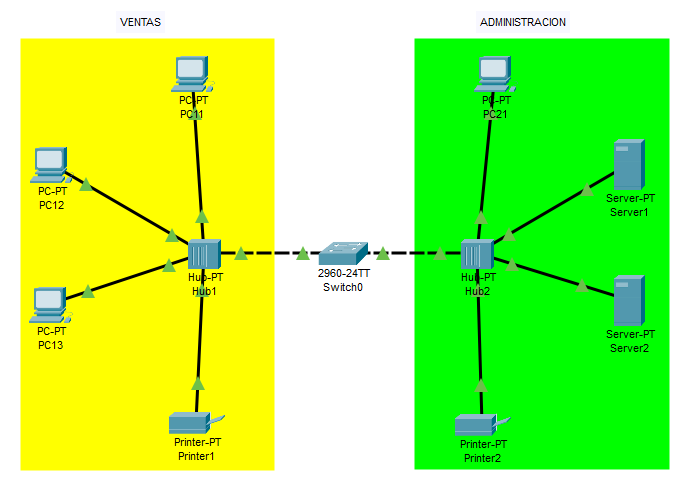
\includegraphics[width=0.85\linewidth]{img_02} 
        \linebreak
        \small {\bfseries Figura 1}: Conexión ventas y administración con Hubs e interconectados a un switch.
    \end{center}
    \pagebreak
    
    \section{El protocolo ARP}
    Lista de direcciones MAC de la figura 2:
    \begin{center}
        \begin{tabular}{| p{3cm} | p{4.1cm} | p{4.1cm} | p{4.1cm} |}
            \hline
            {\bfseries Dispositivo} & {\bfseries Dirección IP} & {\bfseries Dirección MAC} \\\hline
            PC11 & 192.168.1.11 & 0004.9AED.E15B \\\hline
            PC12 & 192.168.1.12 & 000D.BD96.B915 \\\hline
            PC13 & 192.168.1.13 & 0010.114D.79D9 \\\hline
            Printer1 & 192.168.1.14 & 0001.6394.A11E \\\hline
            PC21 & 192.168.1.21 & 0001.96DA.9132 \\\hline
            Server1 & 192.168.1.22 & 00E0.F9A9.3157 \\\hline
            Server2 & 192.168.1.23 & 0000.0C11.2106 \\\hline
            Printer2 & 192.168.1.24 & 00D0.FFED.0B5A \\\hline
        \end{tabular}
    \end{center} 
    
    Realizando el intento de comunicación de PC11 a PC12 a través del comando {\bfseries ping -n 1 192.168.1.12}, la PC11 necesita saber la dirección MAC de PC12, para ello envía un paquete ARP broadcast con la dirección MAC destino FFFF.FFFF.FFFF preguntando quien tiene la IP solicitada. El paquete le llega a todos los dispositivos de la red de, pero solo contesta la PC12 con su información, la cual será registrada por la PC11 en su caché ARP.

    \begin{center}
        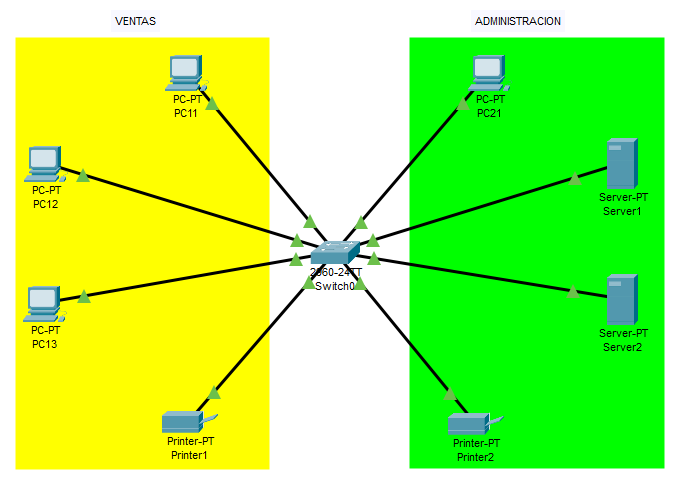
\includegraphics[width=0.85\linewidth]{img_03} 
        \linebreak
        \small {\bfseries Figura 2}: Dispositivos conectados directamente al switch0 con cable utp.
    \end{center}

    Mediante el comando ARP es posible colocar entradas estáticas en la caché ARP. Es utilizado para crear, editar y mostrar las asignaciones de direcciones físicas en un nodo. A continuación veremos la lista de comandos disponibles: \linebreak
    
    \begin{itemize}
        \item {\bfseries arp -a} enumera todos los nodos que se encuentran en la caché ARP.
        \item {\bfseries arp -d 192.168.1.12} eliminará la entrada del nodo {\bfseries 192.168.1.12} de la tabla ARP.
        \item {\bfseries arp -s 192.168.1.12 000D.BD96.B915} agregará a la tabla ARP una entrada para el nodo 192.168.1.12.
    \end{itemize}

    Tener la posibilidad de modificar la tabla ARP puede ser práctica en algunos escenarios, pero también genera problemas de seguridad. Por ejemplo, {\bfseries ARP Spoofing} consiste en enviar mensajes ARP falsos a una red a fin de que se le asigne una dirección IP de esa red de manera legítima. Otro ejemplo, es {\bfseries Man in The Middle (MTM)} que consiste en espiar el tráfico de red de la víctima, utilizando ARP fraudulentos para redireccionar el tráfico a través del ordenador del atacante y enviandolo a destinatario para que parezca que no pasa nada.

    \begin{center}
        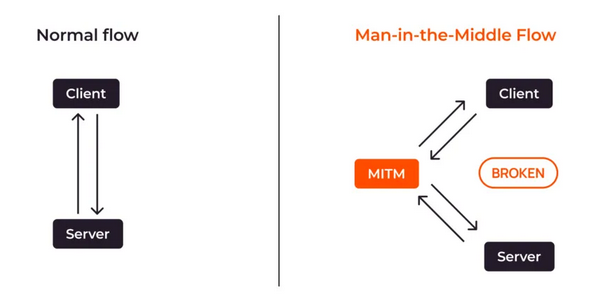
\includegraphics[width=0.85\linewidth]{img_04} 
        \linebreak
        \small {\bfseries Figura 3}: Representación ataque MTM.
    \end{center}

    \section{Switch learning}
    Una vez realizadas algunas pruebas adicionales de comunicación entre los dispositivos conectados al switch de la figura 2 podemos ver como la tabla de direcciones MAC del switch se ha completado con la información de todos los nodos conectados directamente.

    \begin{center}
        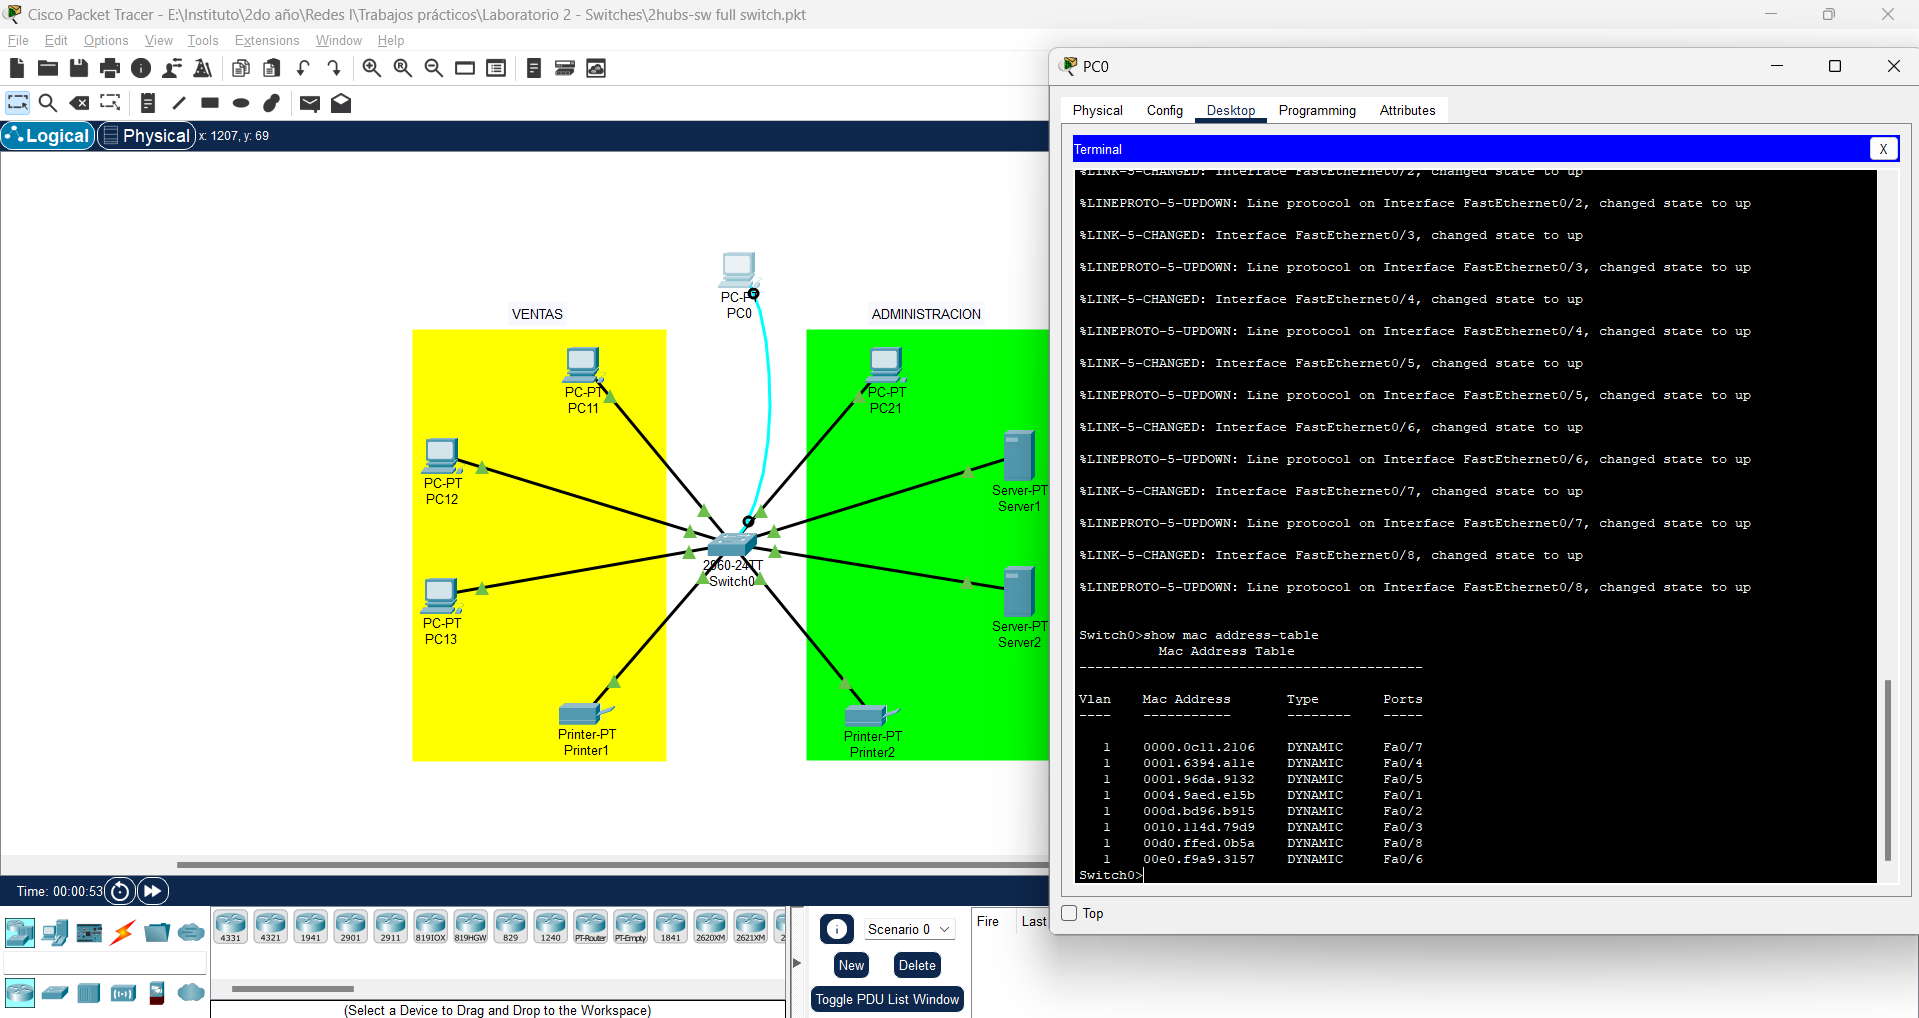
\includegraphics[width=0.85\linewidth]{img_05} 
        \linebreak
        \small {\bfseries Figura 4}: Nodos conectados a switch, pc conectada por consola y tabla de MAC.
    \end{center}

    \pagebreak
    \section{Referencias}
        \begin{itemize}
            \item \href{https://github.com/MarianC312/Laboratorio_2_Switches}{Repositorio GitHub}
            \item \href{https://www.youtube.com/watch?v=5KH_b8RI_Lw}{Router vs Switch: ¿Quién controla el broadcast?}
            \item \href{https://francisconi.org/linux/comandos/arp}{Comandos ARP}
        \end{itemize}
\end{document}